\section[Le Memorie]{Le Memorie}
\label{sec:memory}
\sectionframe{images/covers/cover_sd_memory.png}{Le Memorie}	 


\subsection[Lo scopo delle memorie]{Lo scopo delle memorie}
\begin{frame}
	\frametitle{Lo scopo delle memorie}
	
	\begin{block}{Lo scopo delle memorie}
		La memoria, in informatica, è un elemento di un computer che ha il compito di garantire la persistenza dei dati e/o delle istruzioni dei programmi.\\~\\
		Esistono diversi tipi di memoria e la loro realizzazione fisica dà vita a vari supporti di memorizzazione differenti tra loro.\\~\\
		Ricordiamo che il bit è la più piccola unità di informazione elettronica che possiamo memorizzare.		
		
		
%		La CPU è un'elaborata combinazione di transistor che può essere definita \textit{circuito integrato}.\\~\\
%		\pause
%		All'interno della CPU individuiamo tre elementi fondamentali:
%		\begin{itemize}
%			\item \textbf{la CU}, \textit{Control Unit} (l’unità di controllo):\\
%			coordina l'esecuzione delle operazioni da parte del processore;
%			\item \textbf{la ALU}, \textit{Arithmetic-Logic Unit} (l’Unità Aritmetico-Logica):\\
%			si occupa di eseguire le operazioni aritmetico-logiche;
%			\item \textbf{i registri di memoria}:\\
%			diverse \textit{celle di memoria} dedicate a scopi specifici che vengono utilizzati per il controllo dell'esecuzione di un programma.
%		\end{itemize}
	\end{block}
	
\end{frame}


\subsection[I flip-flop]{I flip-flop}
\begin{frame}
	\frametitle{I flip-flop}
	
	\begin{block}{I flip-flop}
		Esistono diverse tecnologie per la realizzazione dei circuiti di memoria. Uno dei dispositivi elettronici più semplici per la memorizzazione dei bit è il \textbf{flip-flop}. Il flip-flop è una delle possibili implementazioni della cella di memoria elementare.		
	\end{block}
	
	\begin{block}{I flip-flop SR (detti SR Latch)}
		Il \textbf{flip-flop SR}, noto anche come \textbf{SR Latch}, può essere considerato uno dei circuiti logici sequenziali più basilari possibili. Questo semplice flip-flop è fondamentalmente un dispositivo bistabile di memoria a un bit che ha due ingressi:
		\begin{itemize}
			\item \textbf{S}: che prende il nome di \textbf{set}, che imposta l'uscita a 1
			\item \textbf{R}: che prende il nome di \textbf{reset}, che imposta l'uscita a 0
		\end{itemize}
	\end{block}
	
\end{frame}


\subsubsection[Flip-Flop SR - NOR Gate]{Flip-Flop SR - NOR Gate}
\begin{frame}
	\frametitle{Flip-Flop SR - NOR Gate}
	 
	\begin{figure}[!htbp] 
		\centering
		%\advance\leftskip-0.25cm
		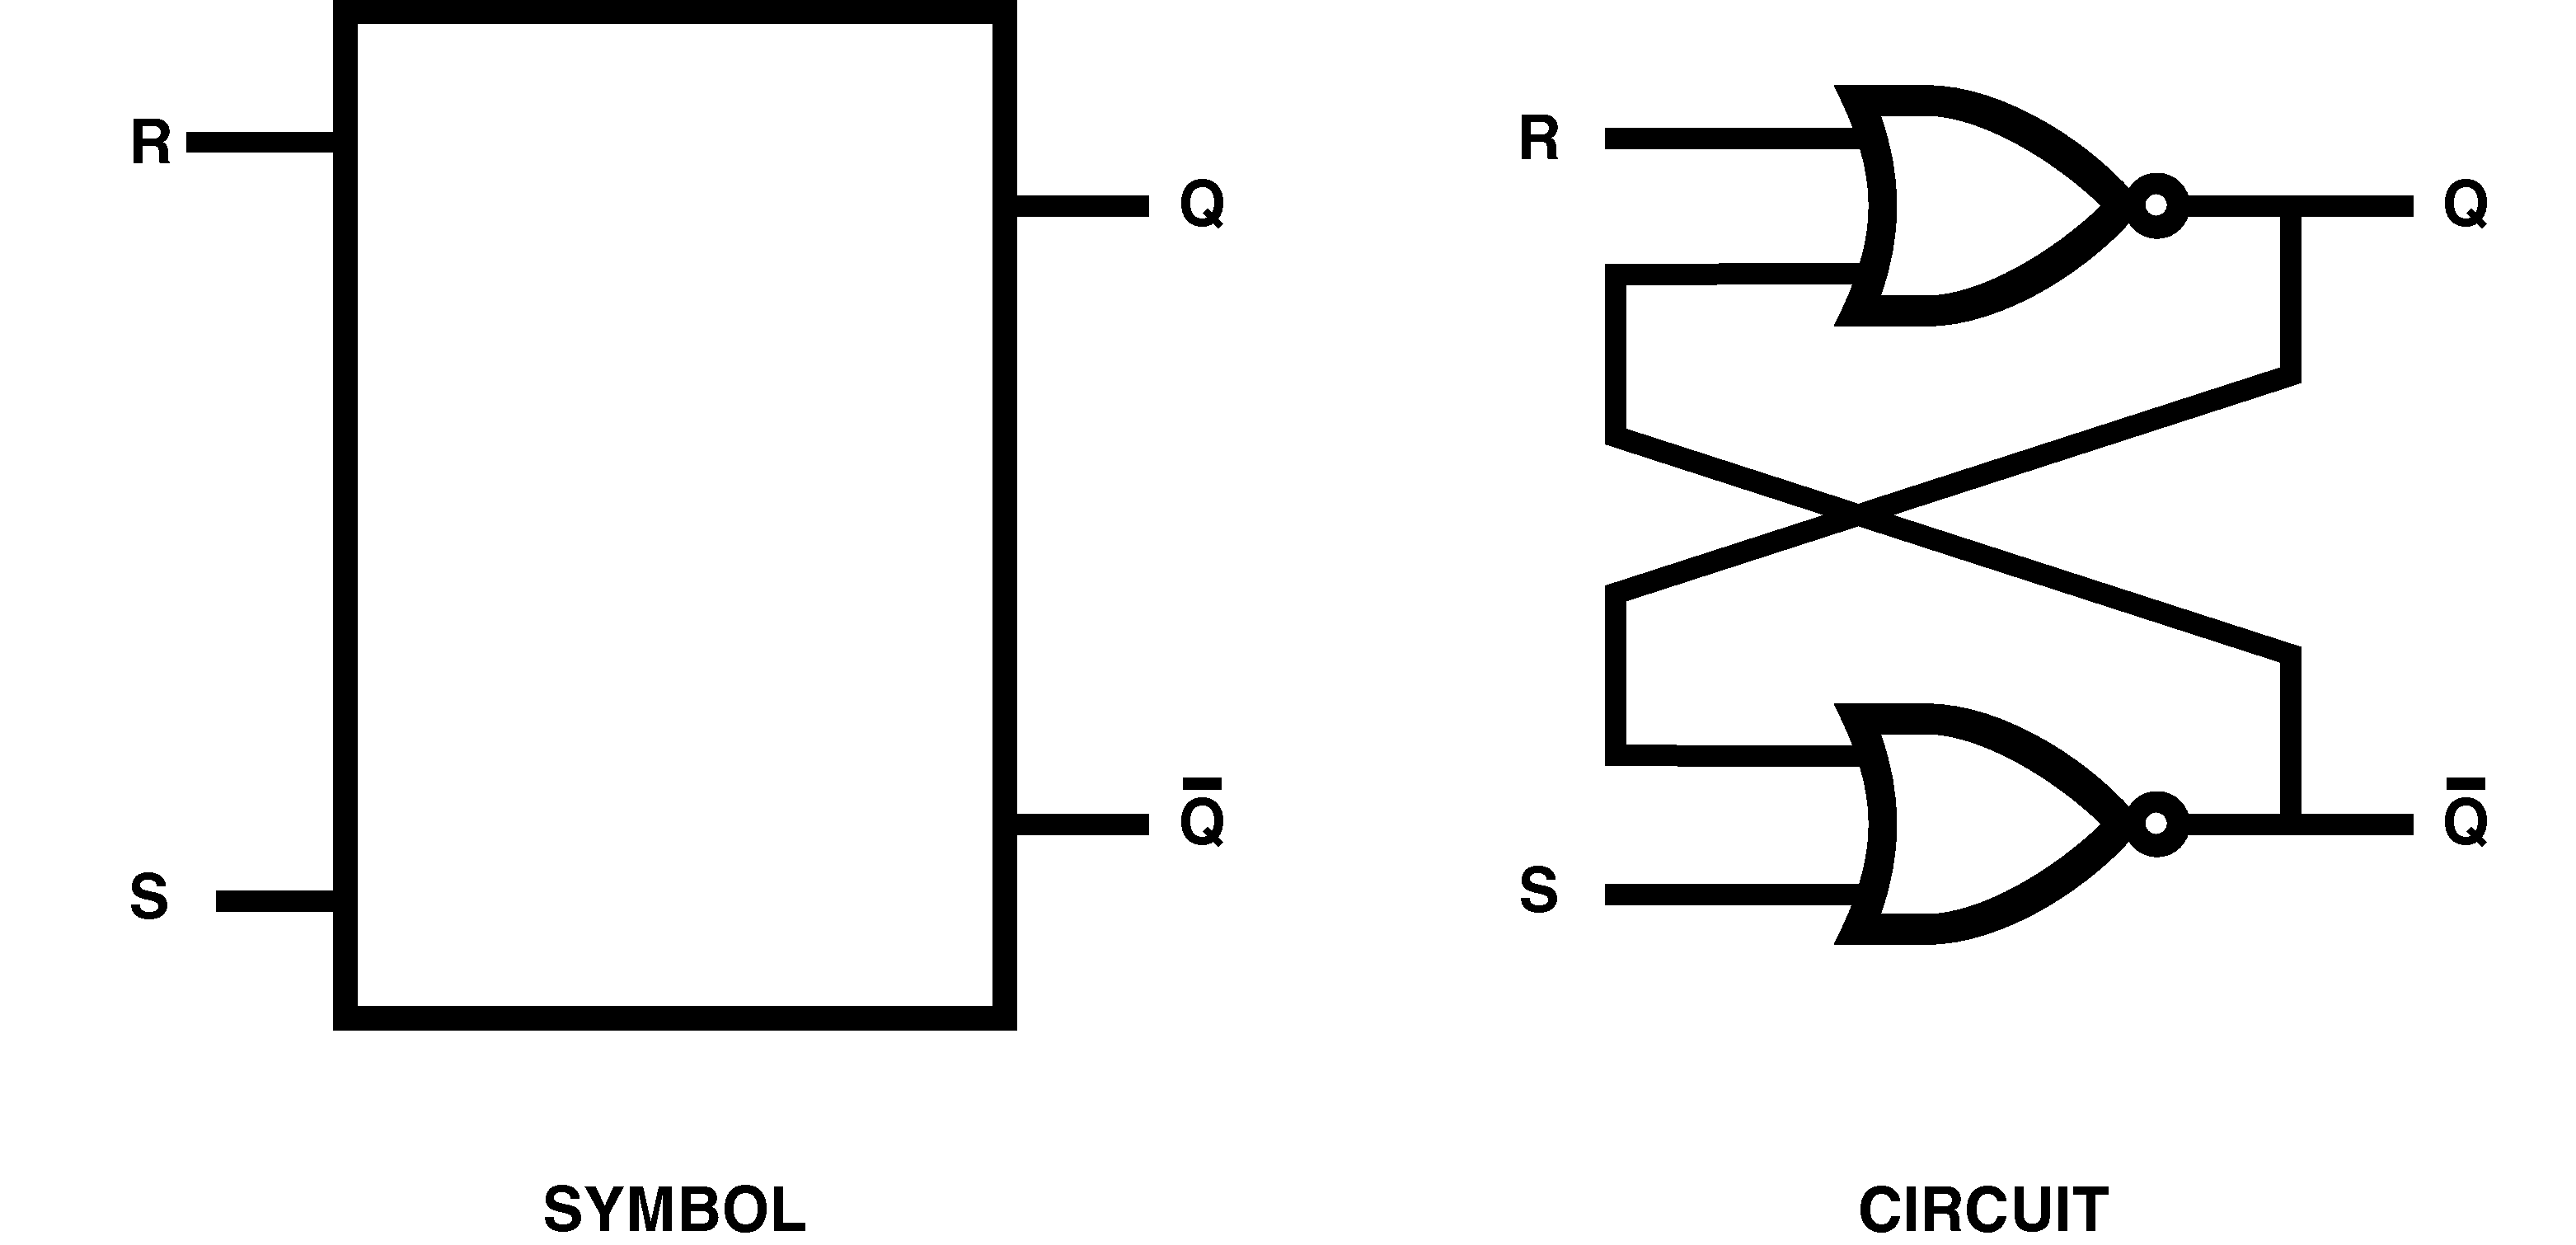
\includegraphics[width=0.95\linewidth]{images/5_memory/flip_flop_sr_nor.pdf}
		\caption{Il flip-flop SR: vedi il \underline{\href{https://www.youtube.com/watch?v=br2pbjAnP2k}{video su youtube}}}
	\end{figure}
	
\end{frame}

\begin{frame}
	\frametitle{Flip-Flop SR - NOR Gate}
	 
	\begin{figure}[!htbp] 
		\centering
		%\advance\leftskip-0.25cm
		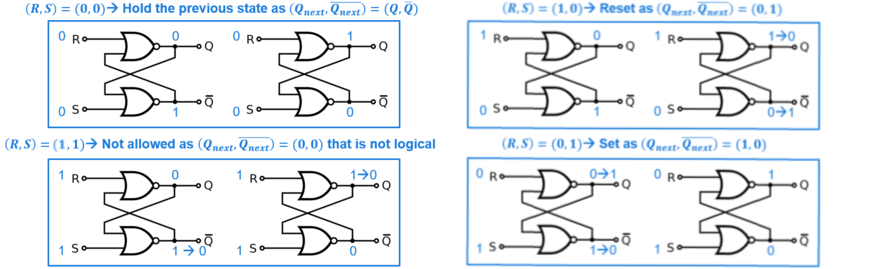
\includegraphics[width=1.0\linewidth]{images/5_memory/flip_flop_sr_nor.png}
		\caption{Il flip-flop SR con NOR, esempi}
	\end{figure}
	
\end{frame}

\begin{frame}

	\frametitle{Flip-Flop SR - NOR Gate}

%	\begin{block}{K-means: algoritmo}
		\centering
		\animategraphics[controls={play, step, stop}, height=7cm]{3.0}{images/5_memory/flip_flop_sr_nor/flip_flop_sr_nor-}{0}{15}
		\label{fig:flip_flop_sr_nor}
%	\end{block}

\end{frame}


\subsubsection[Flip-Flop SR - NAND Gate]{Flip-Flop SR - NAND Gate}
\begin{frame}
	\frametitle{Flip-Flop SR - NAND Gate}
	 
	\begin{figure}[!htbp]  
		\centering
		%\advance\leftskip-0.25cm
		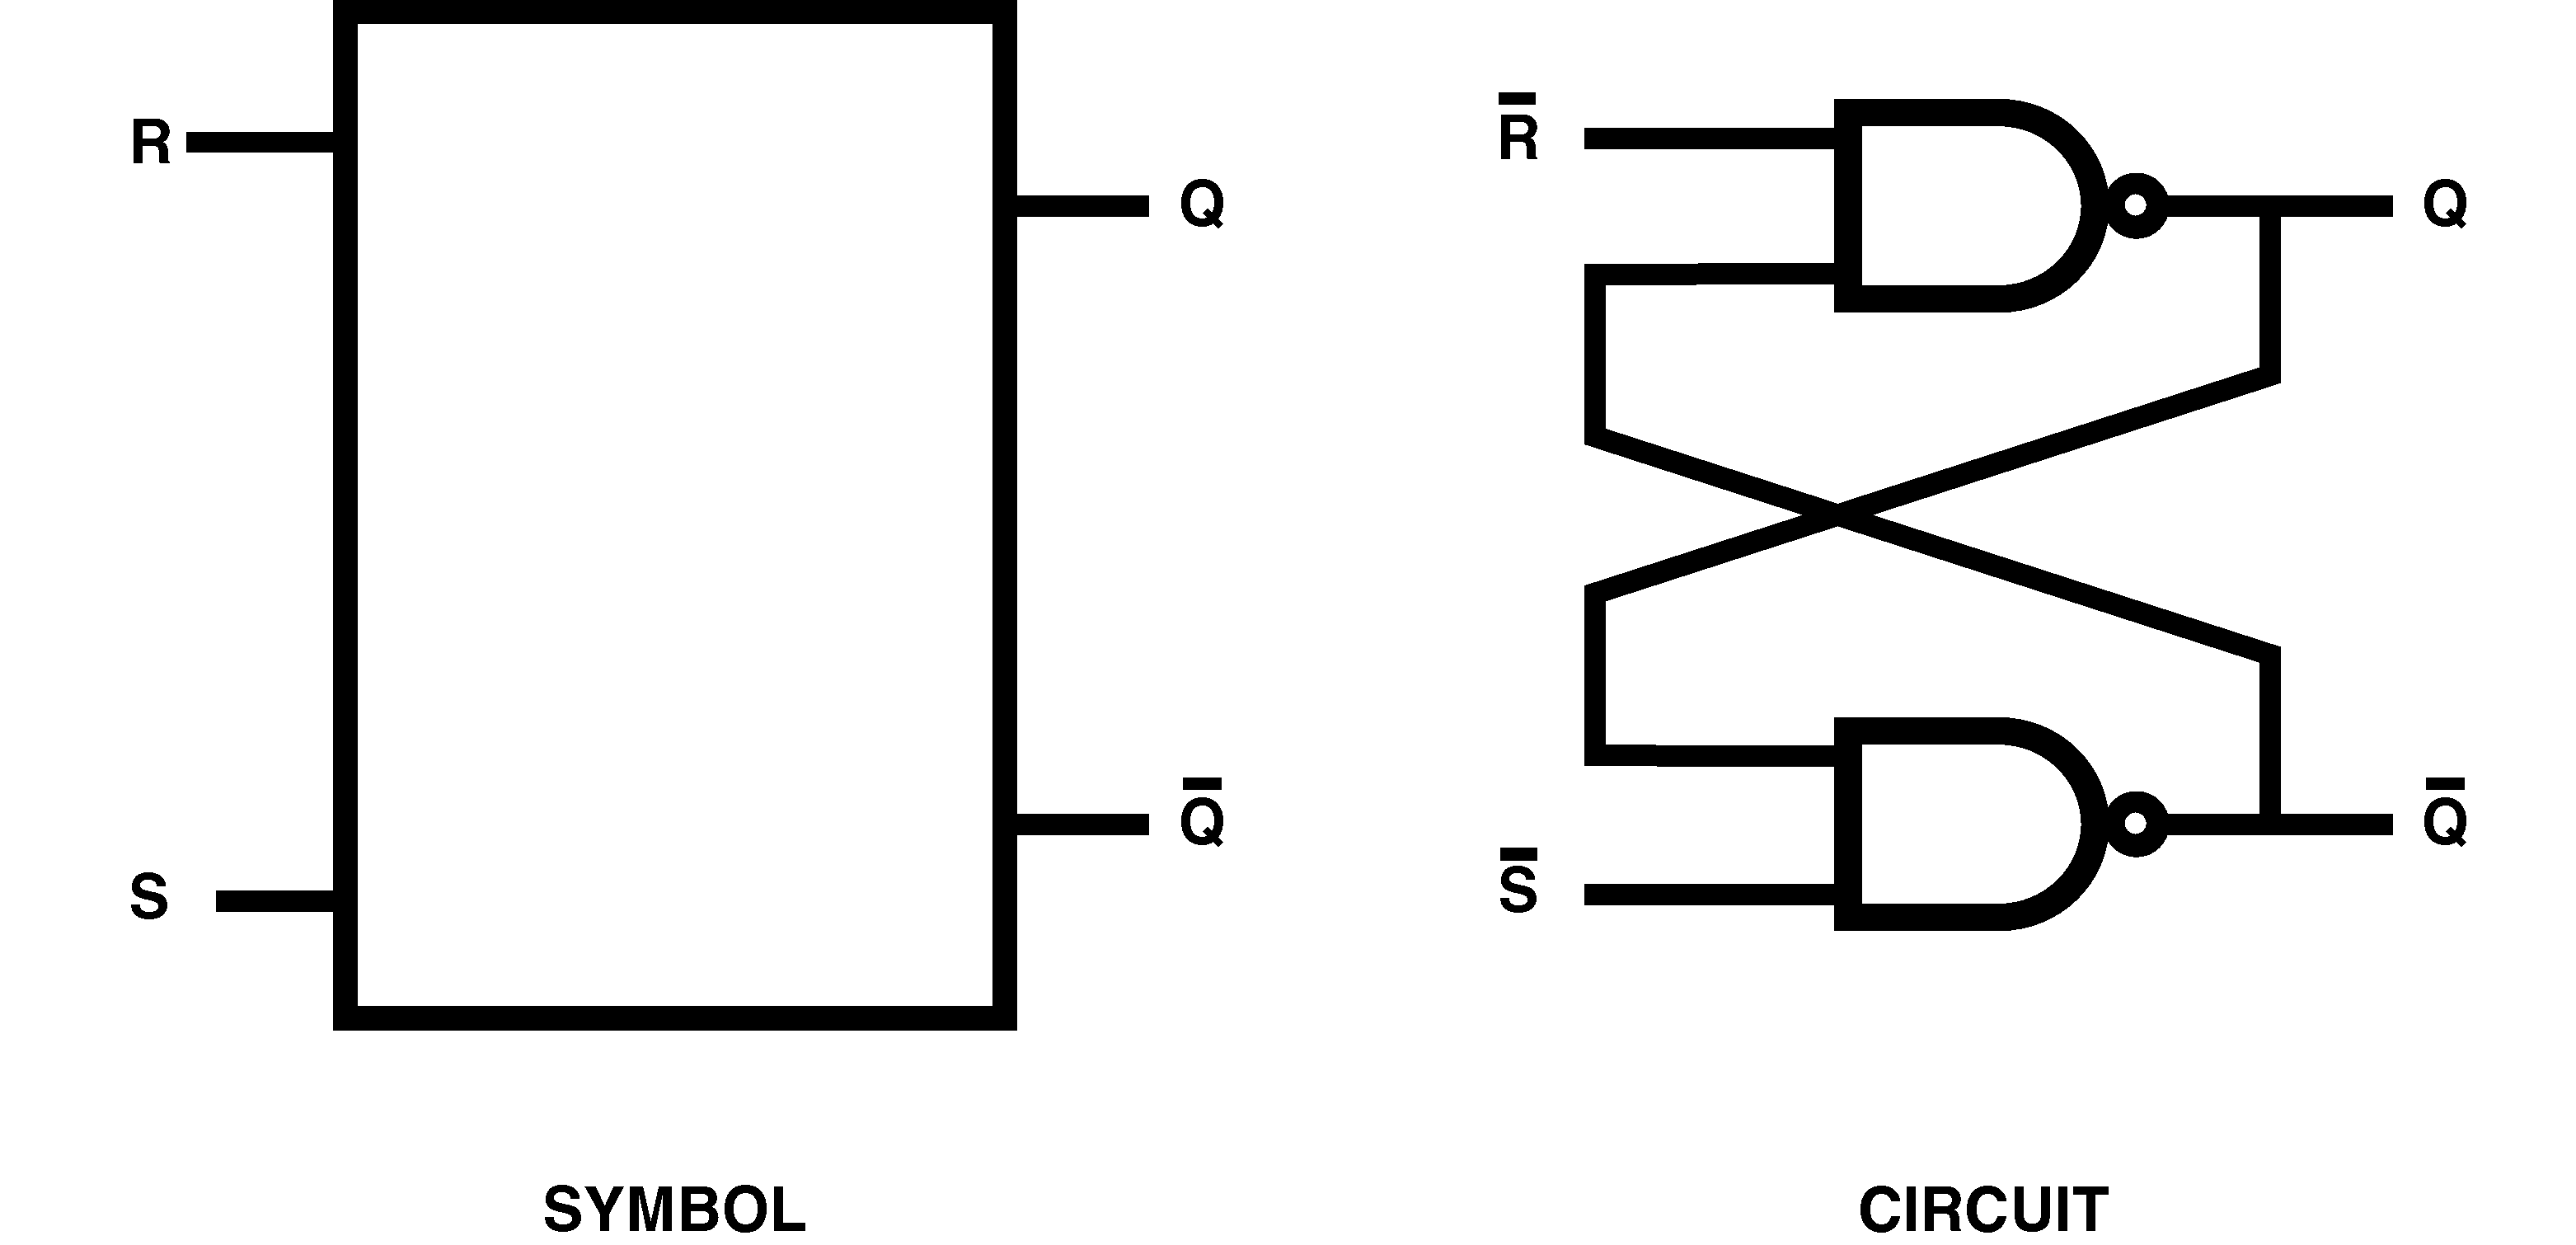
\includegraphics[width=0.95\linewidth]{images/5_memory/flip_flop_sr_nand.pdf}
		\caption{Il flip-flop SR: vedi il \underline{\href{https://www.youtube.com/watch?v=Y9k2oiSJkz4}{video su youtube}}}
	\end{figure}
	
\end{frame}


\subsubsection[Flip-Flop D]{Flip-Flop D}
\begin{frame}
	\frametitle{Flip-Flop D}
	 
	\begin{figure}[!htbp] 
		\centering
		%\advance\leftskip-0.25cm
		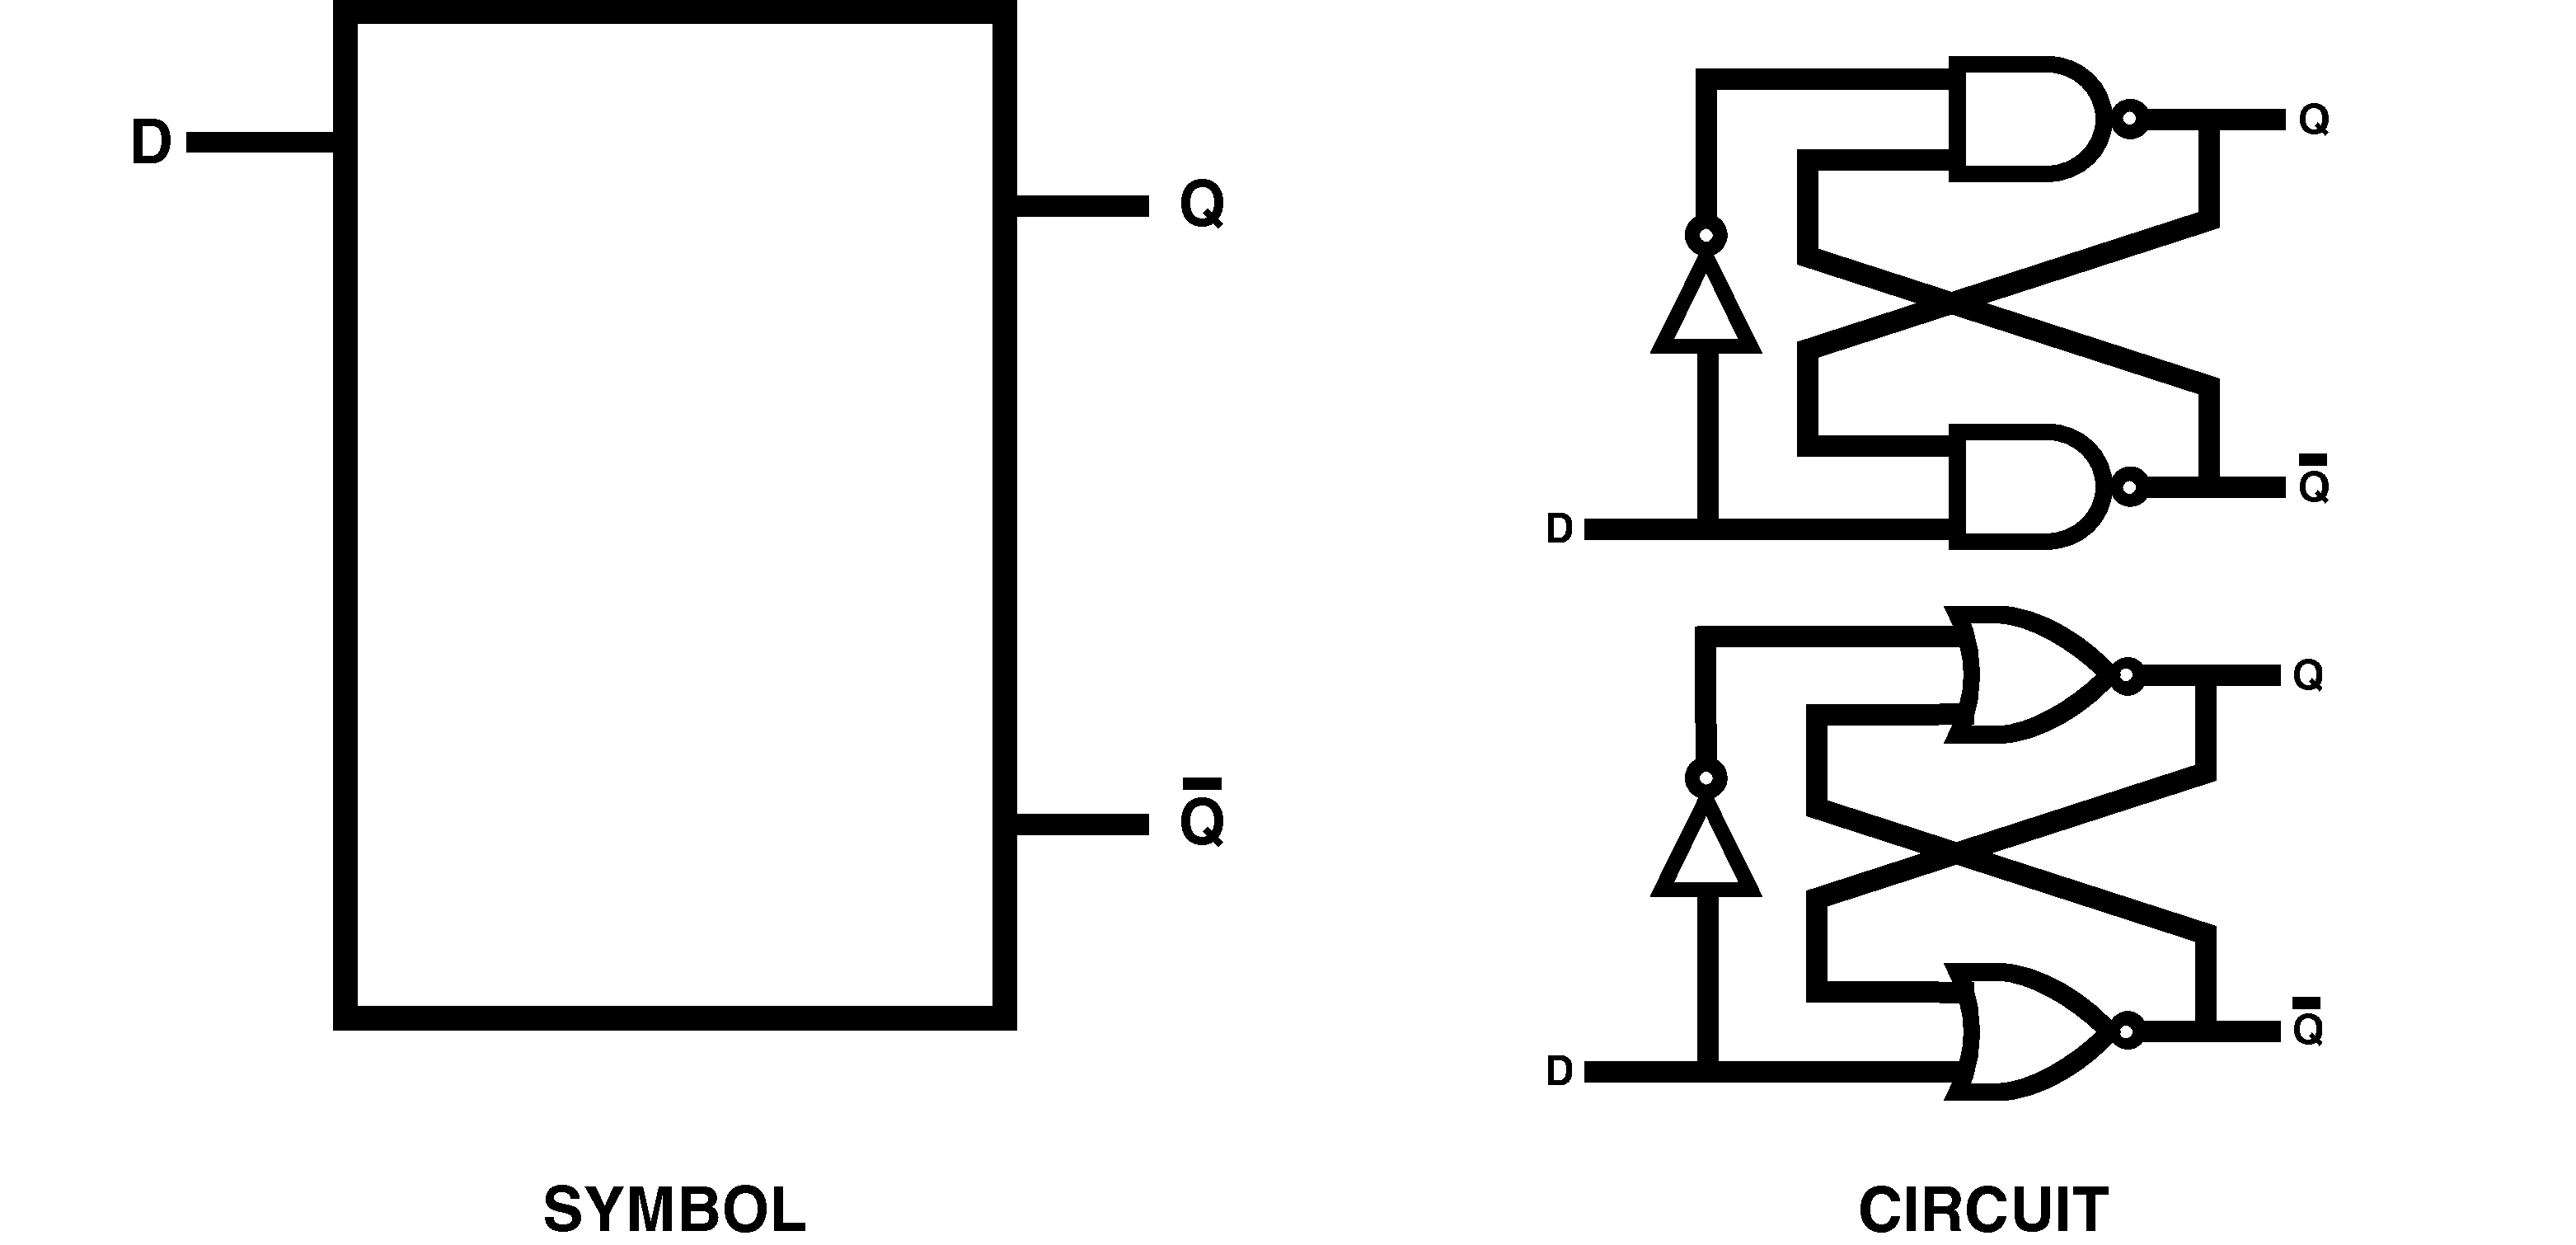
\includegraphics[width=0.95\linewidth]{images/5_memory/flip_flop_d.pdf}
		\caption{Il flip-flop D: è utile per memorizzare un bit di informazione che vengono presentate su una sola line detta "\textbf{Data Line}" (da cui la lettera \textbf{D})}
	\end{figure}
	
\end{frame}


\subsection[Il collo di bottiglia delle memorie]{Il collo di bottiglia delle memorie}
\begin{frame}
	\frametitle{Il collo di bottiglia delle memorie}
	 
	\begin{block}{Il collo di bottiglia}
		Il \textbf{collo di bottiglia} è un fenomeno che si verifica quando le prestazioni di un sistema o le sue capacità sono fortemente vincolate da un singolo componente. Il termine è una metafora del collo di bottiglia reale, che limita il flusso d'uscita dell'acqua.
	\end{block}
	
	\begin{block}{Le prestazioni della memoria RAM}
		Le prestazioni della CPU si sono evolute nel tempo e le prestazioni sono aumentate in maniera esponenziale (vedi \textbf{Legge di Moore}).\\
		Le prestazioni delle memorie non riuscite a tenere il passo con tale ritmo, per questo è stato necessario trovare delle strategie per ridurre al minimo l'impatto di tale collo di bottiglia.
	\end{block}
	
\end{frame}


\subsection[La gerarchia delle memorie]{La gerarchia delle memorie}
\begin{frame}
	\frametitle{Il collo di bottiglia delle memorie}
	 
	\begin{block}{Le prestazioni della memoria RAM}
		Una delle strategie adottate è stata quella di introdurre un sistema gerarchico di memorie.
	\end{block}
	
	\begin{figure}[!htbp] 
		\centering
		%\advance\leftskip-0.25cm
		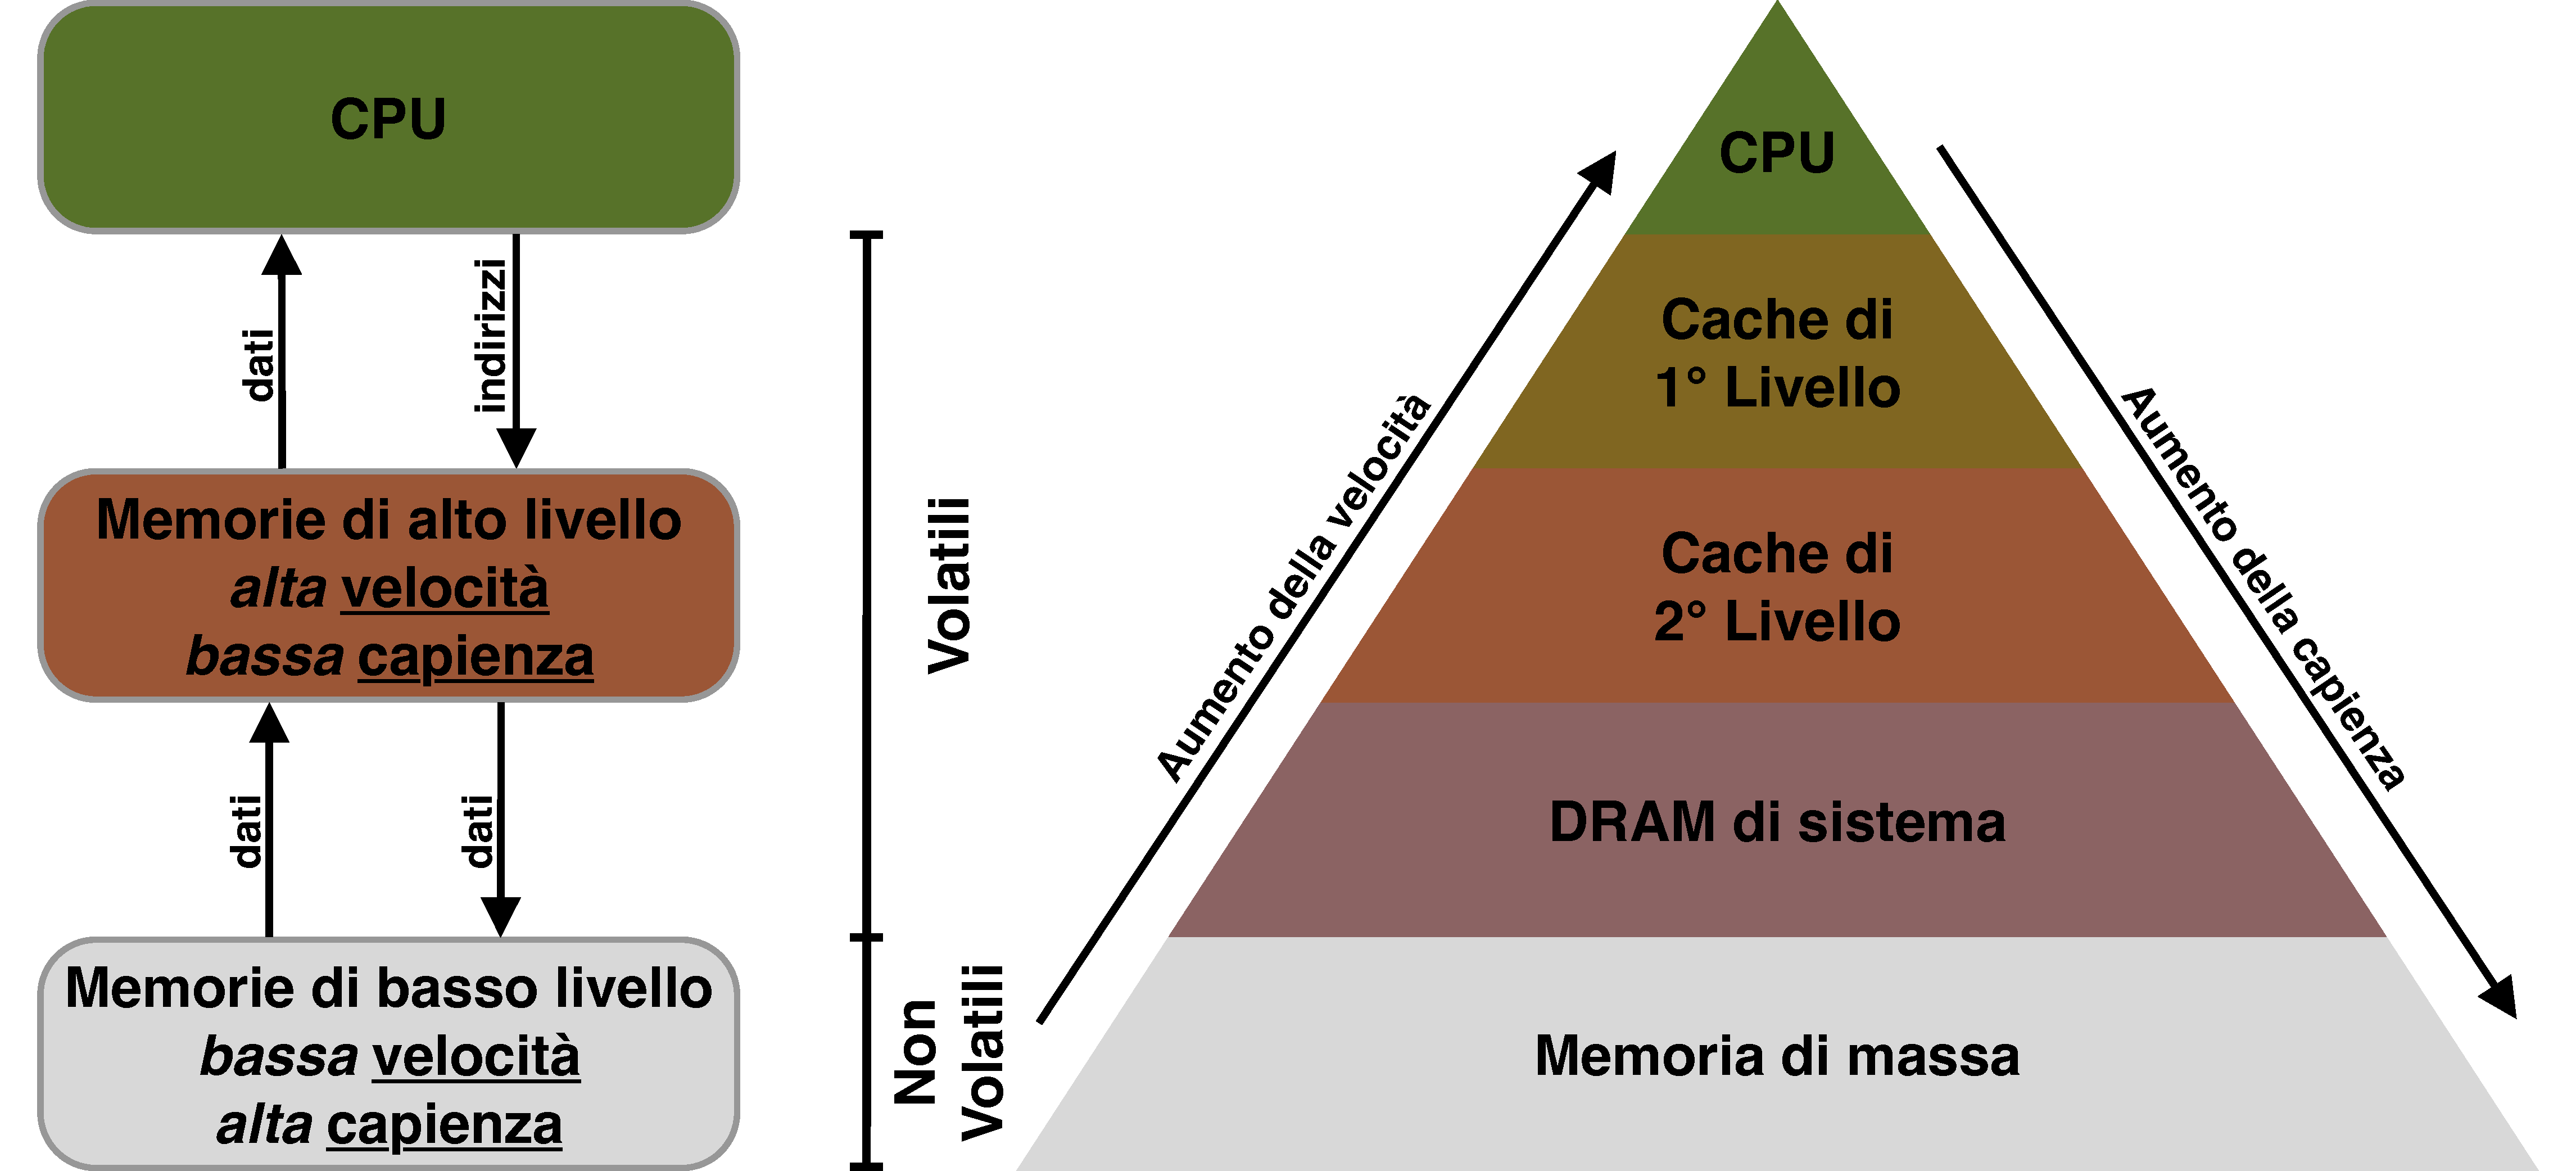
\includegraphics[width=0.8\linewidth]{images/5_memory/memory_hierarchy.pdf}
%		\caption{La CPU: CU, ALU e registri}
		\label{fig:memory_hierarchy}
	\end{figure}
	
\end{frame}



